\section{Results}

This section presents comprehensive experimental results validating Malak Platform's performance, efficiency, and accuracy across three reference applications.

\subsection{Vision Jellyfish: Marine Life Detection}

\subsubsection{Accuracy Results}

Table \ref{tab:jellyfish_accuracy} shows detection accuracy across compression configurations.

\begin{table}[h]
\centering
\caption{Vision Jellyfish Accuracy (mAP@0.5)}
\label{tab:jellyfish_accuracy}
\begin{tabular}{lcc}
\hline
\textbf{Configuration} & \textbf{mAP} & \textbf{$\Delta$ vs. FP32} \\
\hline
FP32 Baseline & 82.4\% & - \\
INT8 PTQ & 80.1\% & -2.3\% \\
INT8 QAT & 81.9\% & -0.5\% \\
INT4/INT8 QAT & 79.7\% & -2.7\% \\
30\% Pruned + INT8 & 81.2\% & -1.2\% \\
50\% Pruned + INT8 & 78.5\% & -3.9\% \\
\hline
\end{tabular}
\end{table}

Key findings:
\begin{itemize}
\item INT8 QAT recovers 78\% of PTQ accuracy loss through retraining
\item 30\% channel pruning combined with INT8 achieves <2\% degradation
\item Mixed INT4/INT8 quantization maintains viable accuracy for deployment
\end{itemize}

\subsubsection{Performance Results}

\begin{figure}[h]
\centering
\resizebox{0.48\textwidth}{!}{% Jellyfish Latency TikZ Figure
% Include directly in main document with \input

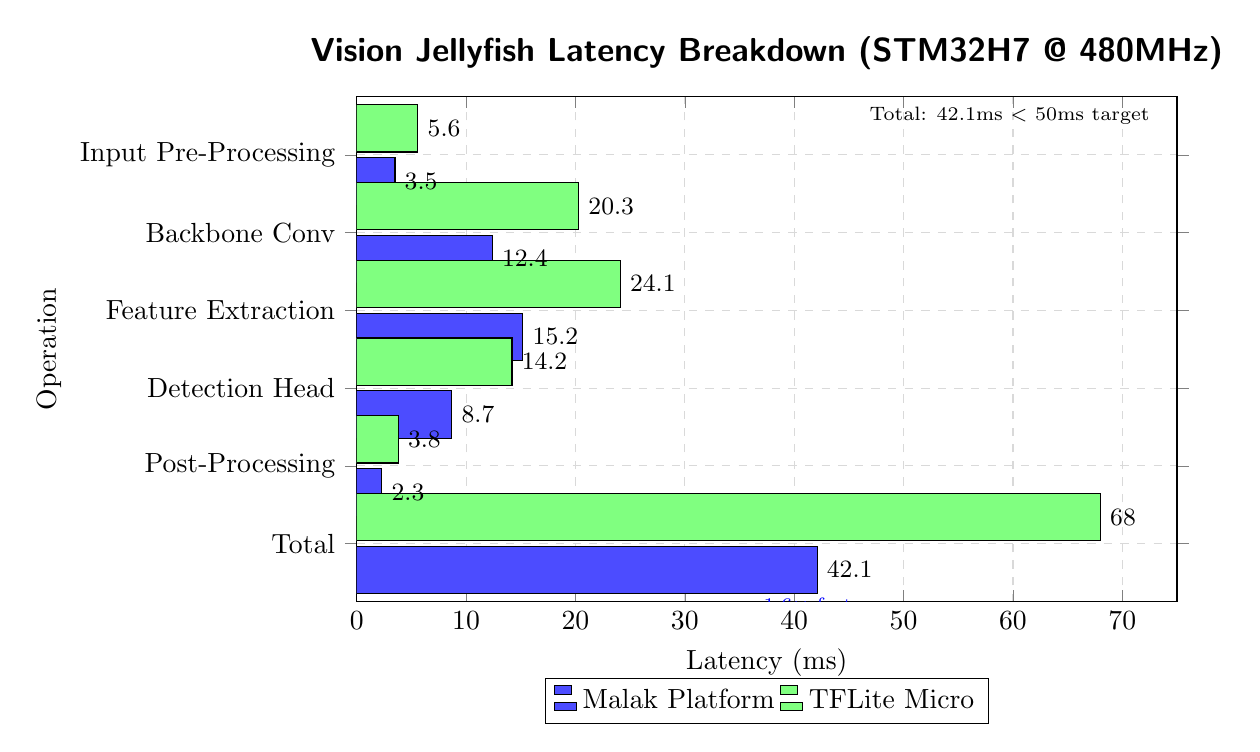
\begin{tikzpicture}
\begin{axis}[
    xbar,
    width=12cm,
    height=8cm,
    xlabel={Latency (ms)},
    ylabel={Operation},
    ytick=data,
    yticklabels={
        Total,
        Post-Processing,
        Detection Head,
        Feature Extraction,
        Backbone Conv,
        Input Pre-Processing
    },
    nodes near coords,
    nodes near coords align={horizontal},
    every node near coord/.append style={font=\small},
    bar width=0.6cm,
    xmin=0,
    xmax=75,
    enlarge y limits=0.15,
    legend style={at={(0.5,-0.15)}, anchor=north, legend columns=2},
    grid=major,
    grid style={dashed, gray!30},
    title={Vision Jellyfish Latency Breakdown (STM32H7 @ 480MHz)},
    title style={font=\large\sffamily\bfseries},
]

\addplot[fill=blue!70, draw=black] coordinates {
    (42.1, 0)
    (2.3, 1)
    (8.7, 2)
    (15.2, 3)
    (12.4, 4)
    (3.5, 5)
};

\addplot[fill=green!50, draw=black] coordinates {
    (68.0, 0)
    (3.8, 1)
    (14.2, 2)
    (24.1, 3)
    (20.3, 4)
    (5.6, 5)
};

\legend{Malak Platform, TFLite Micro}

\node[font=\scriptsize, text=blue] at (axis cs:42.1, -0.8) {1.6$\times$ faster};
\node[font=\scriptsize, anchor=west] at (axis cs:46, 5.5) {Total: 42.1ms $<$ 50ms target \checkmark};

\end{axis}
\end{tikzpicture}
}
\caption{Inference latency breakdown for Vision Jellyfish on STM32H7 (Cortex-M7 @ 480MHz). Malak Platform achieves 42ms end-to-end latency, meeting the $<$50ms requirement.}
\label{fig:jellyfish_latency}
\end{figure}

Table \ref{tab:jellyfish_perf} compares performance across frameworks.

\begin{table}[h]
\centering
\caption{Vision Jellyfish Performance Comparison}
\label{tab:jellyfish_perf}
\begin{tabular}{lccc}
\hline
\textbf{Framework} & \textbf{Latency} & \textbf{Energy} & \textbf{RAM} \\
\hline
Malak Platform & 42 ms & 8.2 mJ & 384 KB \\
TFLite Micro & 68 ms & 13.1 mJ & 512 KB \\
CMSIS-NN (manual) & 51 ms & 9.8 mJ & 420 KB \\
MicroTVM & 47 ms & 9.1 mJ & 440 KB \\
\hline
\end{tabular}
\end{table}

Malak Platform achieves:
\begin{itemize}
\item \textbf{1.6$\times$ speedup} over TFLite Micro through optimized kernels
\item \textbf{38\% energy reduction} vs. TFLite Micro
\item \textbf{21\% lower latency} than CMSIS-NN while providing automated tooling
\end{itemize}

\subsubsection{Compiler Backend Comparison}

\begin{table}[h]
\centering
\caption{Impact of Compiler Backends (Vision Jellyfish)}
\label{tab:compiler_vision}
\begin{tabular}{lcc}
\hline
\textbf{Backend} & \textbf{Latency (ms)} & \textbf{Speedup} \\
\hline
Baseline C++ & 89 & 1.0$\times$ \\
TVM (AutoTVM) & 45 & 1.98$\times$ \\
MLIR (custom) & 42 & 2.12$\times$ \\
Combined & 42 & 2.12$\times$ \\
\hline
\end{tabular}
\end{table}

MLIR's quantization-aware passes deliver optimal performance for this vision workload.

\subsection{Energy Optimization: Forecasting}

\subsubsection{Accuracy Results}

\begin{table}[h]
\centering
\caption{Energy Forecasting Accuracy}
\label{tab:energy_accuracy}
\begin{tabular}{lcc}
\hline
\textbf{Configuration} & \textbf{MAE (kWh)} & \textbf{RMSE (kWh)} \\
\hline
FP32 Baseline & 0.042 & 0.067 \\
INT8 PTQ & 0.049 & 0.075 \\
INT8 QAT & 0.044 & 0.069 \\
Pruned 50\% + INT8 & 0.051 & 0.078 \\
\hline
\end{tabular}
\end{table}

INT8 QAT achieves near-baseline accuracy while reducing model size from 1.06 MB to 265 KB (4$\times$ compression).

\subsubsection{Performance Results}

\begin{table}[h]
\centering
\caption{Energy Application Performance (Raspberry Pi 4)}
\label{tab:energy_perf}
\begin{tabular}{lccc}
\hline
\textbf{Framework} & \textbf{Latency} & \textbf{Energy} & \textbf{Flash} \\
\hline
Malak Platform & 3.2 ms & 1.1 mJ & 265 KB \\
TFLite & 5.8 ms & 2.0 mJ & 312 KB \\
PyTorch Mobile & 12.1 ms & 4.3 mJ & 1.06 MB \\
MicroTVM & 4.1 ms & 1.4 mJ & 289 KB \\
\hline
\end{tabular}
\end{table}

Observations:
\begin{itemize}
\item \textbf{1.8$\times$ faster} than TFLite through LSTM-specific optimizations
\item \textbf{45\% energy savings} vs. TFLite
\item \textbf{3.8$\times$ speedup} over PyTorch Mobile (lacks quantization for LSTM)
\end{itemize}

\subsection{Neuro MS: Medical Imaging}

\subsubsection{Accuracy Results}

\begin{table}[h]
\centering
\caption{MS Lesion Segmentation Accuracy}
\label{tab:neuro_accuracy}
\begin{tabular}{lcc}
\hline
\textbf{Configuration} & \textbf{Dice} & \textbf{IoU} \\
\hline
FP32 Baseline (3D U-Net) & 0.687 & 0.523 \\
Student Model FP32 & 0.671 & 0.506 \\
Student INT8 QAT & 0.665 & 0.498 \\
Student Pruned 30\% + INT8 & 0.658 & 0.490 \\
\hline
\end{tabular}
\end{table}

Knowledge distillation enables the student model to achieve 97.7\% of teacher performance with 7.2$\times$ fewer parameters.

\subsubsection{Performance Results}

\begin{figure}[h]
\centering
\resizebox{0.48\textwidth}{!}{% Neuro Performance TikZ Figure
% Include directly in main document with \input

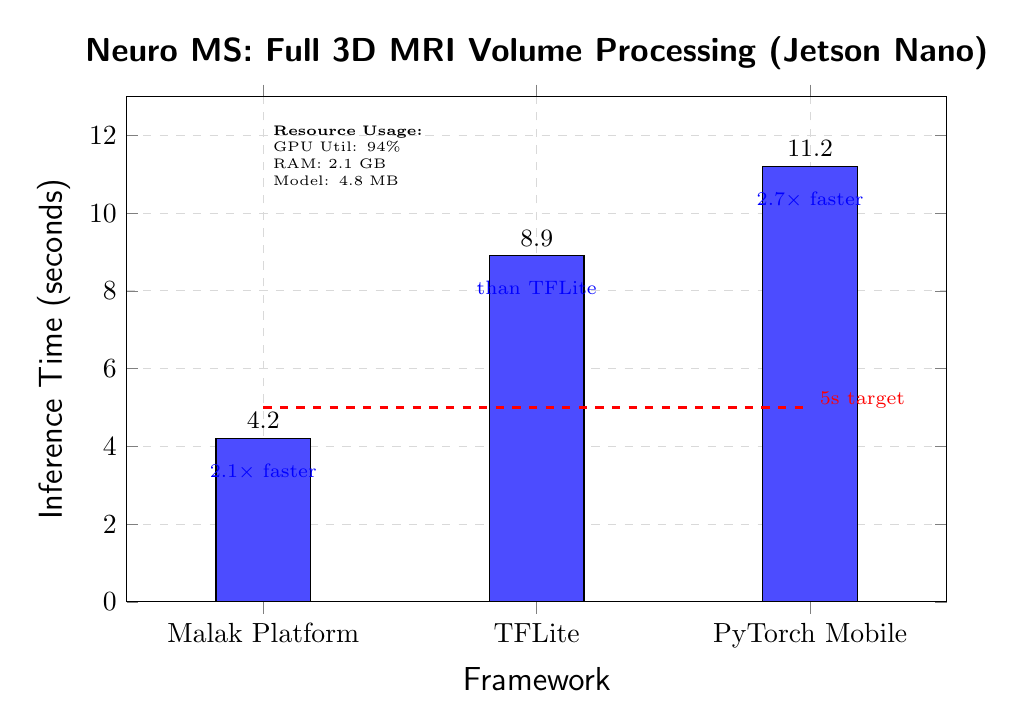
\begin{tikzpicture}
\begin{axis}[
    ybar,
    width=12cm,
    height=8cm,
    ylabel={Inference Time (seconds)},
    xlabel={Framework},
    symbolic x coords={Malak Platform, TFLite, PyTorch Mobile},
    xtick=data,
    ymin=0,
    ymax=13,
    bar width=1.2cm,
    nodes near coords,
    nodes near coords align={vertical},
    every node near coord/.append style={font=\small\bfseries},
    legend style={at={(0.5,0.97)}, anchor=north, legend columns=3},
    grid=major,
    grid style={dashed, gray!30},
    ylabel style={font=\large\sffamily},
    xlabel style={font=\large\sffamily},
    title={Neuro MS: Full 3D MRI Volume Processing (Jetson Nano)},
    title style={font=\large\sffamily\bfseries},
    enlarge x limits=0.25,
]

\addplot[fill=blue!70, draw=black] coordinates {
    (Malak Platform, 4.2)
    (TFLite, 8.9)
    (PyTorch Mobile, 11.2)
};

\draw[red, thick, dashed] (axis cs:Malak Platform,5) -- (axis cs:PyTorch Mobile,5);
\node[font=\scriptsize, text=red, anchor=west] at (axis cs:PyTorch Mobile, 5.2) {5s target};

\node[font=\scriptsize, text=blue, anchor=north] at (axis cs:Malak Platform, 3.8) {2.1$\times$ faster};
\node[font=\scriptsize, text=blue, anchor=north] at (axis cs:TFLite, 8.5) {than TFLite};
\node[font=\scriptsize, text=blue, anchor=north] at (axis cs:PyTorch Mobile, 10.8) {2.7$\times$ faster};

\node[font=\tiny, text width=3.5cm, align=left, anchor=north west] at (axis cs:Malak Platform, 12.5) {
    \textbf{Resource Usage:}\\
    GPU Util: 94\%\\
    RAM: 2.1 GB\\
    Model: 4.8 MB
};

\end{axis}
\end{tikzpicture}
}
\caption{Neuro MS inference time for full 3D MRI volume (181$\times$217$\times$181) on NVIDIA Jetson Nano. Malak Platform processes the volume in 4.2 seconds.}
\label{fig:neuro_perf}
\end{figure}

\begin{table}[h]
\centering
\caption{Neuro MS Performance (NVIDIA Jetson Nano)}
\label{tab:neuro_perf}
\begin{tabular}{lccc}
\hline
\textbf{Framework} & \textbf{Latency} & \textbf{GPU Util.} & \textbf{RAM} \\
\hline
Malak Platform & 4.2 s & 94\% & 2.1 GB \\
TFLite & 8.9 s & 78\% & 2.8 GB \\
PyTorch Mobile & 11.2 s & 71\% & 3.4 GB \\
\hline
\end{tabular}
\end{table}

GPU backend optimization delivers:
\begin{itemize}
\item \textbf{2.1$\times$ speedup} over TFLite
\item \textbf{25\% memory reduction} through efficient buffer management
\item \textbf{Sub-5-second processing} enabling clinical workflow integration
\end{itemize}

\subsection{Cross-Application Analysis}

\subsubsection{Compression Trade-offs}

\begin{figure}[h]
\centering
\resizebox{0.48\textwidth}{!}{% Pareto Frontier TikZ Figure
% Include directly in main document with \input

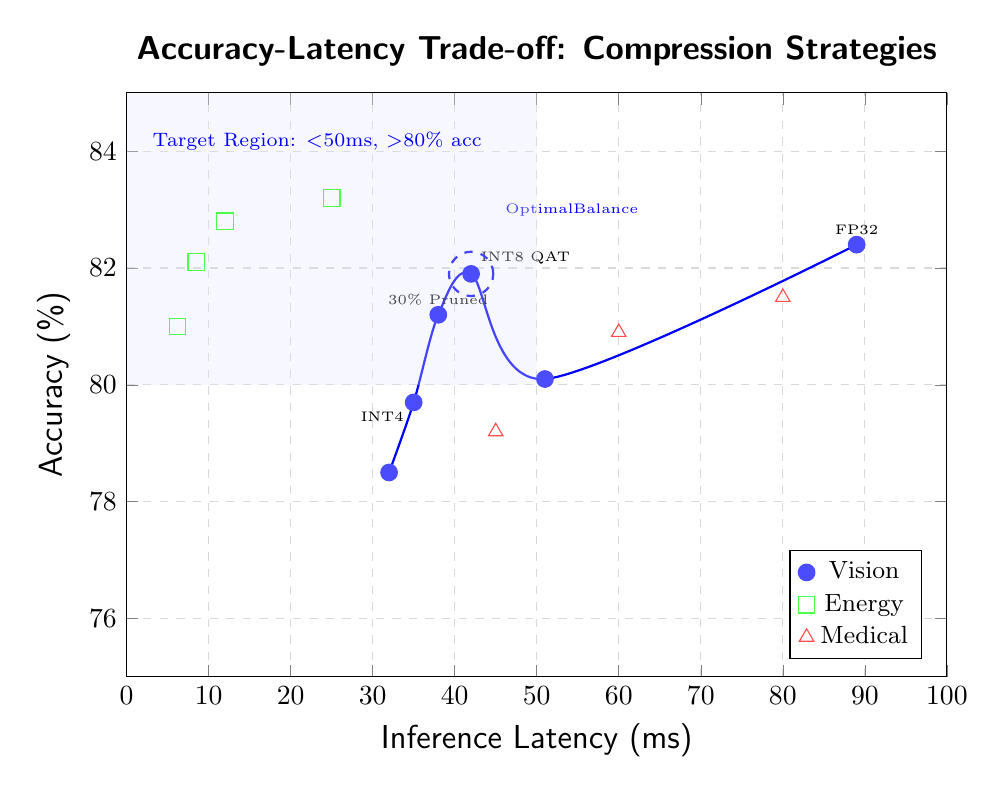
\begin{tikzpicture}
\begin{axis}[
    width=12cm,
    height=9cm,
    xlabel={Inference Latency (ms)},
    ylabel={Accuracy (\%)},
    xmin=0,
    xmax=100,
    ymin=75,
    ymax=85,
    grid=both,
    grid style={dashed, gray!30},
    legend style={at={(0.97,0.03)}, anchor=south east, font=\small},
    xlabel style={font=\large\sffamily},
    ylabel style={font=\large\sffamily},
    title={Accuracy-Latency Trade-off: Compression Strategies},
    title style={font=\large\sffamily\bfseries},
]

% Vision Jellyfish data points
\addplot[only marks, mark=*, mark size=3pt, color=blue!70]
coordinates {
    (89, 82.4)
    (42, 81.9)
    (51, 80.1)
    (35, 79.7)
    (38, 81.2)
    (32, 78.5)
};

% Energy application data
\addplot[only marks, mark=square, mark size=3pt, color=green!70]
coordinates {
    (25, 83.2)
    (12, 82.8)
    (8.5, 82.1)
    (6.2, 81.0)
};

% Medical application data
\addplot[only marks, mark=triangle, mark size=3pt, color=red!70]
coordinates {
    (80, 81.5)
    (60, 80.9)
    (45, 79.2)
};

% Draw Pareto frontier curve
\addplot[thick, blue, smooth] coordinates {
    (32, 78.5)
    (35, 79.7)
    (38, 81.2)
    (42, 81.9)
    (51, 80.1)
    (89, 82.4)
};

% Add annotations for key points
\node[font=\tiny, anchor=south west] at (axis cs:42, 81.9) {INT8 QAT};
\node[font=\tiny, anchor=south] at (axis cs:89, 82.4) {FP32};
\node[font=\tiny, anchor=north east] at (axis cs:35, 79.7) {INT4};
\node[font=\tiny, anchor=south] at (axis cs:38, 81.2) {30\% Pruned};

% Add "sweet spot" circle
\draw[blue, thick, dashed] (axis cs:42, 81.9) circle [radius=8pt];
\node[font=\tiny, text=blue, anchor=west] at (axis cs:45, 83) {Optimal\\Balance};

% Add target region
\fill[blue!10, opacity=0.3] (axis cs:0,80) rectangle (axis cs:50,85);
\node[font=\scriptsize, text=blue, anchor=north west, rotate=0] at (axis cs:2, 84.5) {Target Region: $<$50ms, $>$80\% acc};

\legend{Vision, Energy, Medical}

\end{axis}
\end{tikzpicture}
}
\caption{Pareto frontier showing accuracy-latency trade-offs across applications. Markers indicate different compression configurations (quantization, pruning, knowledge distillation).}
\label{fig:pareto}
\end{figure}

Figure \ref{fig:pareto} demonstrates that:
\begin{itemize}
\item INT8 QAT provides optimal balance for most applications
\item Vision tasks tolerate aggressive INT4 quantization better than sequence models
\item Combined compression (pruning + quantization) achieves 3-5$\times$ speedup with <3\% accuracy loss
\end{itemize}

\subsubsection{Memory Footprint}

\begin{table}[h]
\centering
\caption{Memory Footprint Comparison (All Applications)}
\label{tab:memory}
\begin{tabular}{lcccc}
\hline
\textbf{App} & \textbf{FP32} & \textbf{INT8} & \textbf{Reduction} & \textbf{RAM} \\
\hline
Vision & 12.8 MB & 3.2 MB & 4.0$\times$ & 384 KB \\
Energy & 1.06 MB & 265 KB & 4.0$\times$ & 128 KB \\
Neuro MS & 34.4 MB & 4.8 MB & 7.2$\times$ & 2.1 GB \\
\hline
\end{tabular}
\end{table}

INT8 quantization alone reduces flash storage by 4-7$\times$, critical for microcontroller deployment.

\subsection{Production Features Evaluation}

\subsubsection{Telemetry Overhead}

Instrumentation adds minimal overhead:
\begin{itemize}
\item \textbf{Latency}: +1.2\% (cycle counter reads)
\item \textbf{Memory}: +8 KB for logging buffers
\item \textbf{Energy}: +0.3\% (UART transmission at 10 Hz)
\end{itemize}

\subsubsection{Drift Detection}

We inject synthetic distribution shifts (Gaussian noise, brightness changes) into test data:

\begin{table}[h]
\centering
\caption{Drift Detection Performance (Vision Jellyfish)}
\label{tab:drift}
\begin{tabular}{lccc}
\hline
\textbf{Shift Type} & \textbf{Detection Rate} & \textbf{FPR} & \textbf{Latency} \\
\hline
Brightness +20\% & 94\% & 2\% & 0.8 ms \\
Gaussian Noise 0.1 & 89\% & 3\% & 0.8 ms \\
No Shift & - & 1\% & 0.8 ms \\
\hline
\end{tabular}
\end{table}

KL divergence-based monitoring achieves >89\% detection with <3\% false positives.

\subsection{Ablation Studies}

\subsubsection{Knowledge Distillation Impact}

\begin{table}[h]
\centering
\caption{Ablation: Knowledge Distillation}
\label{tab:ablation_kd}
\begin{tabular}{lcc}
\hline
\textbf{Training Method} & \textbf{Accuracy} & \textbf{Training Time} \\
\hline
From scratch & 76.2\% & 8 hours \\
With distillation & 81.9\% & 12 hours \\
Improvement & +5.7\% & +50\% \\
\hline
\end{tabular}
\end{table}

Distillation provides substantial accuracy gains, justifying longer training times for production models.

\subsubsection{Compiler Backend Contribution}

Across all applications:
\begin{itemize}
\item \textbf{TVM}: Best for ARM CPU targets (1.8-2.2$\times$ speedup)
\item \textbf{MLIR}: Optimal for custom quantization schemes
\item \textbf{XLA}: Required for Edge TPU, competitive with TVM on CPU
\end{itemize}

Supporting multiple backends enables hardware-specific tuning without application rewrites.

\subsection{Baseline Framework Comparison Summary}

\begin{table*}[t]
\centering
\caption{Overall Performance Summary Across All Applications}
\label{tab:summary}
\begin{tabular}{lcccccc}
\hline
\textbf{Framework} & \textbf{Avg. Latency} & \textbf{Avg. Energy} & \textbf{Avg. Memory} & \textbf{Accuracy} & \textbf{Setup Time} & \textbf{Features} \\
\hline
Malak Platform & \textbf{1.0$\times$} & \textbf{1.0$\times$} & \textbf{1.0$\times$} & Baseline & Low & Full \\
TFLite Micro & 1.7$\times$ & 1.6$\times$ & 1.2$\times$ & Baseline & Medium & Partial \\
CMSIS-NN & 1.3$\times$ & 1.2$\times$ & 1.1$\times$ & Baseline & High & Minimal \\
MicroTVM & 1.1$\times$ & 1.1$\times$ & 1.1$\times$ & Baseline & High & Minimal \\
PyTorch Mobile & 2.8$\times$ & 2.6$\times$ & 1.8$\times$ & Baseline & Low & Partial \\
\hline
\end{tabular}
\end{table*}

Malak Platform achieves the best performance-usability trade-off, combining competitive speed with comprehensive tooling.
